
\begin{frame}{‌الگوریتم بلمن-فورد}
\begin{itemize}\itemr
\item[-]
الگوریتم بلمن-فورد
\fn{1}{Bellman-Ford algorithm}
مسئله کوتاهترین مسیر را در حالت کلی حل می‌کند وقتی وزن یال‌ها می‌توانند منفی نیز باشند.
\item[-]
به ازای یک گراف دلخواه
\m{G = (V,E)}
با یال‌های وزن‌دار و رأس مبدأ
\m{s}
و تابع وزن
\m{w : E \rightarrow \RR}
الگوریتم بلمن فورد در صورتی که یک دور با وزن منفی وجود داشته باشد که از مبدأ قابل دسترسی باشد، مقدار نادرست را باز می‌گرداند، بدین معنی که کوتاهترین مسیر وجود ندارد. اما اگر چنین دوری وجود نداشته باشد، الگوریتم بلمن فورد کوتاهترین مسیر را از مبدأ به همهٔ رئوس را باز می‌گرداند.
\end{itemize}
\end{frame}


\begin{frame}{‌الگوریتم بلمن-فورد}
\begin{itemize}\itemr
\item[-]
الگوریتم بلمن فورد در زیر توصیف شده است.
\begin{algorithm}[H]\alglr
  \caption{Bellman-Ford} 
  \begin{algorithmic}[1]
   \Func{Bellman-Ford}{G,w,s}
   \State Initialize-Single-Source(G, s)
   \For{i = 1 \To |G.V| - 1}
   		\For{each edge (u,v) $\in$ G.E}
   				\State Relax(u,v,w)
   		\EndFor
   	\EndFor
   	\For{each edge (u,v) $\in$ G.E}
   			\If{v.d > u.d + w(u,v)}
   					\State \Return False
   			\EndIf
   	\EndFor
   	\State \Return True                         
  \end{algorithmic}
  \label{alg:merge}
\end{algorithm}
\end{itemize}
\end{frame}


\begin{frame}{‌الگوریتم بلمن-فورد}
\begin{itemize}\itemr
\item[-]
یک مثال از اجرای الگوریتم بلمن فورد در زیر نشان داده شده است.
\begin{figure}
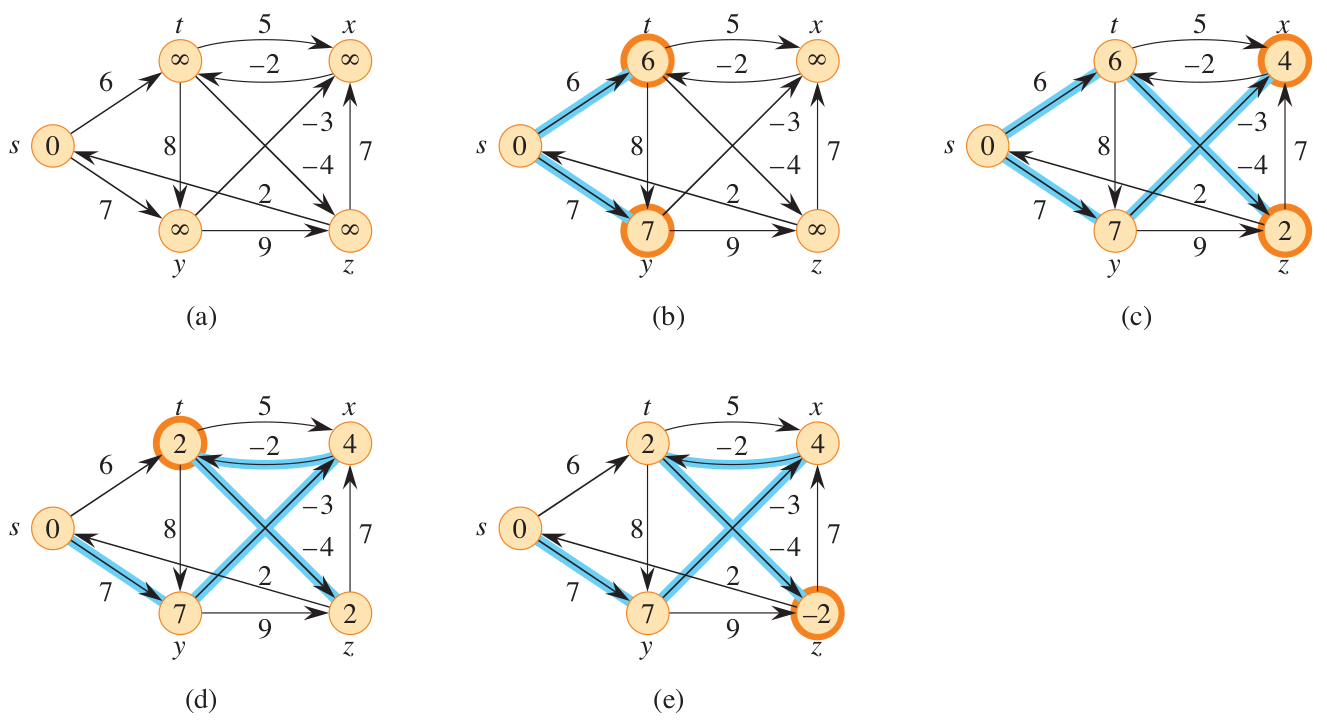
\includegraphics[width=0.7\textwidth]{figs/chap07/613-bellman}
\end{figure}
\end{itemize}
\end{frame}


\begin{frame}{‌الگوریتم بلمن-فورد}
\begin{itemize}\itemr
\item[-]
مقداردهی اولیه در خط ۱ در زمان
\ath{|V|}
اجرا می‌شود.
\item[-]
%اگر گراف با لیست مجاورت نمایش داده شود،
بررسی همهٔ یال‌ها به زمان 
\ath{|E|}
نیاز خواهد داشت.
% وقتی که گراف با لیست مجاورت نمایش داده شده باشد.
\item[-]
در حلقه خطوط ۲ تا ۴ هر یک از
\m{|V| -1}
تکرارهای حلقه، در زمان
\ath{|E|}
اجرا می‌شود.
\item[-]
حلقه خطوط ۵ تا ۷ در زمان
\ath{|E|}
اجرا می‌شود.
\item[-]
بنابراین الگوریتم بلمن فورد در زمان
\m{O(|V| |E|)}
اجرا می‌شود.

\end{itemize}
\end{frame}

\begin{frame}{‌الگوریتم بلمن-فورد}
\begin{itemize}\itemr
\item[-]
برای اثبات درستی الگوریتم بلمن فورد نشان می‌دهیم اگر هیچ دوری با وزن منفی وجود نداشته باشد، این الگوریتم به درستی کوتاهترین مسیر را برای همهٔ رئوس از یک رأس مبدأ محاسبه می‌کند.
\item[-]
قضیه:
فرض کنید
\m{G = (V,E)}
یک گراف وزن‌دار جهت‌دار با رأس مبدأ
\m{s}
و تابع وزن
\m{w : E \rightarrow \RR}
باشد و فرض کنید
\m{G}
هیچ دوری با وزن منفی نداشته باشد که از
\m{s}
قابل دسترسی باشد. آنگاه بعد از
\m{|V| -1}
تکرار در حلقهٔ خطوط ۲ تا ۴ الگوریتم بلمن فورد به دست می‌آوریم
\m{v.d = \delta(s,v)}
به ازای همه رئوس
\m{v}
که از
\m{s}
قابل دسترس هستند.
\end{itemize}
\end{frame}


\begin{frame}{‌الگوریتم بلمن-فورد}
\begin{itemize}\itemr
\item[-]
اثبات : یک رأس
\m{v}
را در نظر بگیرید که از
\m{s}
قابل دسترس است و فرض کنید
\m{p = \langle v_0,v_1, \cdots , v_k \rangle}
به طوری‌که
\m{v_0 = s}
و
\m{v_k = v}
و
\m{p}
کوتاهترین مسیر از
\m{s}
به
\m{v}
باشد.
\item[-]
از آنجایی که کوتاهترین مسیر باید یک مسیر ساده باشد،
\m{p}
حداکثر
\m{|V| -1}
یال دارد و بنابراین
\m{k \leqslant |V| -1} .
\item[-]
هر یک از
\m{|V| -1}
تکرار در حلقه خطوط ۲ تا ۴ همه
\m{|E|}
یال را آزادسازی می‌کند.
\end{itemize}
\end{frame}


\begin{frame}{‌الگوریتم بلمن-فورد}
\begin{itemize}\itemr
\item[-]
بعد از یک بار تکرار حلقه، یال
\m{(s,v_1)}
آزاد سازی می‌شود و بنابراین
\m{v_1.d = w(s,v_1) = \delta(s, v_1)}
وزن کوتاهترین مسیر از
\m{s}
به
\m{v_1}
خواهد بود.
\item[-]
بعد از دو بار تکرار حلقه، یال
\m{(v_1,v_2)}
برای بار دوم آزادسازی می‌شود
 بنابراین
\m{v_2.d = v_1.d + w(v_1,v_2) = \delta(s,v_2)}
وزن کوتاهترین مسیر از
\m{s}
به
\m{v_2}
خواهد بود.
\item[-]
بنابراین
 در تکرار
\m{i}
ام، به ازای
\m{i = 1,2, \cdots, k}
یال
\m{(v_{i-1},v_i)}
 آزادسازی می‌شود و  
\m{v_i.d = v_{i-1}.d + w(v_{i-1},v_i) = \delta(s, v_i)}
وزن کوتاهترین مسیر از
\m{s}
به
\m{v_i}
خواهد بود.
\item[-]
 پس از 
\m{|V| -1}
بار آزادسازی یال‌ها
به دست می‌آوریم:
\begin{align*}
\m{v_k.d = \delta(s,v_k)}
\end{align*}
\end{itemize}
\end{frame}


\iffalse
\begin{frame}{‌الگوریتم بلمن-فورد}
\begin{itemize}\itemr
\item[-]
ویژگی آزادسازی مسیر
\fn{1}{path relaxation property}
به صورت زیر است.
\item[-]
اگر
\m{p = \langle v_0,v_1, \cdots , v_k \rangle}
کوتاهترین مسیر از
\m{s = v_0}
به
\m{v_k}
باشد و یال‌های
\m{p}
به ترتیب
\m{(v_0,v_1)}
،
\m{(v_1,v_2)}
،
\m{\cdots}
،
\m{(v_{k-1},v_k)}
آزادسازی شوند، آنگاه
\m{v_{k}.d = \delta(s,v_k)}
\end{itemize}
\end{frame}
\fi